\documentclass{beamer}
\mode<presentation>
\usepackage{amsmath}
\usepackage{amssymb}
%\usepackage{advdate}
\usepackage{adjustbox}
\usepackage{subcaption}
\usepackage{enumitem}
\usepackage{multicol}
\usepackage{mathtools}
\usepackage{listings}
\usepackage{float}
\usepackage{graphicx}
\usepackage{url}
\def\UrlBreaks{\do\/\do-}
\usetheme{Boadilla}
\usecolortheme{lily}
\setbeamertemplate{footline}
{
  \leavevmode%
  \hbox{%
  \begin{beamercolorbox}[wd=\paperwidth,ht=2.25ex,dp=1ex,right]{author in head/foot}%
    \insertframenumber{} / \inserttotalframenumber\hspace*{2ex} 
  \end{beamercolorbox}}%
  \vskip0pt%
}
\setbeamertemplate{navigation symbols}{}

\providecommand{\nCr}[2]{\,^{#1}C_{#2}} % nCr
\providecommand{\nPr}[2]{\,^{#1}P_{#2}} % nPr
\providecommand{\mbf}{\mathbf}
\providecommand{\pr}[1]{\ensuremath{\Pr\left(#1\right)}}
\providecommand{\qfunc}[1]{\ensuremath{Q\left(#1\right)}}
\providecommand{\sbrak}[1]{\ensuremath{{}\left[#1\right]}}
\providecommand{\lsbrak}[1]{\ensuremath{{}\left[#1\right.}}
\providecommand{\rsbrak}[1]{\ensuremath{{}\left.#1\right]}}
\providecommand{\brak}[1]{\ensuremath{\left(#1\right)}}
\providecommand{\lbrak}[1]{\ensuremath{\left(#1\right.}}
\providecommand{\rbrak}[1]{\ensuremath{\left.#1\right)}}
\providecommand{\cbrak}[1]{\ensuremath{\left\{#1\right\}}}
\providecommand{\lcbrak}[1]{\ensuremath{\left\{#1\right.}}
\providecommand{\rcbrak}[1]{\ensuremath{\left.#1\right\}}}
\theoremstyle{remark}
\newtheorem{rem}{Remark}
\newcommand{\sgn}{\mathop{\mathrm{sgn}}}
\providecommand{\abs}[1]{\left\vert#1\right\vert}
\providecommand{\res}[1]{\Res\displaylimits_{#1}} 
\providecommand{\norm}[1]{\lVert#1\rVert}
\providecommand{\mtx}[1]{\mathbf{#1}}
\providecommand{\mean}[1]{E\left[ #1 \right]}
\providecommand{\fourier}{\overset{\mathcal{F}}{ \rightleftharpoons}}
%\providecommand{\hilbert}{\overset{\mathcal{H}}{ \rightleftharpoons}}
\providecommand{\system}{\overset{\mathcal{H}}{ \longleftrightarrow}}
	%\newcommand{\solution}[2]{\textbf{Solution:}{#1}}
%\newcommand{\solution}{\noindent \textbf{Solution: }}
\providecommand{\dec}[2]{\ensuremath{\overset{#1}{\underset{#2}{\gtrless}}}}
\newcommand{\myvec}[1]{\ensuremath{\begin{pmatrix}#1\end{pmatrix}}}
\let\vec\mathbf

\lstset{
language=C,
frame=single, 
breaklines=true,
columns=fullflexible
}

\numberwithin{equation}{section}

\title{Presentation - Matgeo}
\author{Aryansingh Sonaye \\
AI25BTECH11032 \\
EE1030 - Matrix Theory}

\date{\today} 
\begin{document}

\begin{frame}
\titlepage
\end{frame}

\section{Problem}
\begin{frame}
\frametitle{Problem Statement}
\textbf{Problem 12.6}

Compute the 4-point Discrete Fourier Transform (DFT) of the sequence
\begin{align}
x[n] = \{1,0,2,3\}, \quad n=0,1,2,3.
\end{align}


\end{frame}

\section{Solution}
\subsection{Description of Variables used}
\begin{frame}
\frametitle{Description of Variables used}
\begin{table}[H]
\centering
\begin{tabular}{|c|c|c|}
\hline
\textbf{Symbol} & \textbf{Description} & \textbf{Value} \\
\hline
$N$ & Length of sequence & $4$ \\
\hline
$x[n]$ & Input sequence & $\{1,0,2,3\}$ \\
\hline
$W_N$ & Twiddle factor & $e^{-j2\pi/N}$ \\
\hline
\end{tabular}
\caption{} \label{}
\end{table}


\end{frame}

\subsection{Theoretical Solution }

\begin{frame}
\frametitle{Theoretical Solution}
The $N$-point DFT is defined as
\begin{align}
    X[k] &= \sum_{n=0}^{N-1} x[n] \, W_N^{kn}, \quad k=0,1,\dots,N-1,
\end{align}
where
\begin{align}
    W_N = e^{-j \tfrac{2\pi}{N}}.
\end{align}

For $N=4$,
\begin{align}
    W_4 = e^{-j \tfrac{2\pi}{4}} = -j,
\end{align}
so that
\begin{align}
    W_4^0 = 1, \quad W_4^1 = -j, \quad W_4^2 = -1, \quad W_4^3 = j.
\end{align}

\end{frame}

\begin{frame}
\frametitle{Theoretical Solution}
The DFT matrix is
\begin{align}
F_4 = \myvec{
1 & 1 & 1 & 1 \\
1 & -j & -1 & j \\
1 & -1 & 1 & -1 \\
1 & j & -1 & -j
}.
\end{align}

The input vector is
\begin{align}
\vec{x} = \myvec{1 \\ 0 \\ 2 \\ 3}.
\end{align}

Thus,
\begin{align}
\vec{X} &= F_4 \, \vec{x}.
\end{align}

\end{frame}

\begin{frame}
\frametitle{Theoretical Solution}
Row-by-row computation:
\begin{align}
X[0] &= 1+0+2+3 = 6, \\
X[1] &= 1 + 0(-j) - 2 + 3j = -1+3j, \\
X[2] &= 1 + 0(-1) + 2 - 3 = 0, \\
X[3] &= 1 + 0(j) - 2 - 3j = -1-3j.
\end{align}

Therefore, the DFT vector is
\begin{align}
\vec{X} = \myvec{6 \\ -1+3j \\ 0 \\ -1-3j}.
\end{align}

\section*{Final Answer}
\begin{align}
\vec{X} = \myvec{6 \\ -1+3j \\ 0 \\ -1-3j}
\end{align}

\end{frame}


\subsection{Plot}
\begin{frame}
    \frametitle{Plot}
\begin{figure}[H]
   \centering
   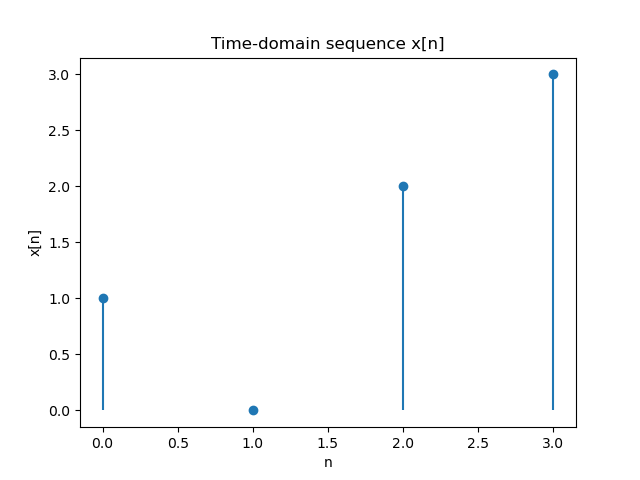
\includegraphics[width=0.8\columnwidth]{figs/fig3.png}
   \caption{}
   \label{}
   \end{figure}
\end{frame}

\begin{frame}
    \frametitle{Plot}
\begin{figure}[H]
   \centering
   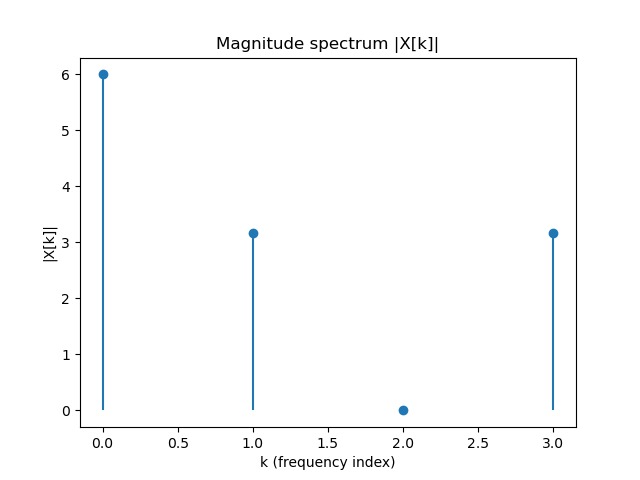
\includegraphics[width=0.8\columnwidth]{figs/fig4.png}
   \caption{}
   \label{}
   \end{figure}
\end{frame}

\begin{frame}
    \frametitle{Plot}
\begin{figure}[H]
   \centering
   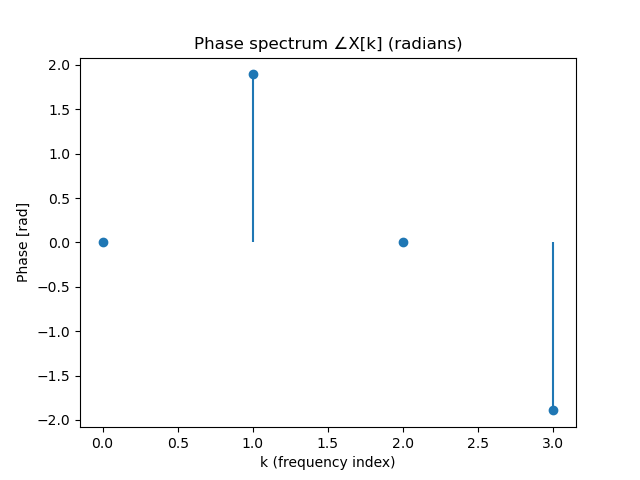
\includegraphics[width=0.8\columnwidth]{figs/fig5.png}
   \caption{}
   \label{}
   \end{figure}
\end{frame}

\begin{frame}[fragile]
    \frametitle{Code - C}
    \begin{lstlisting}
#include <math.h>

#ifndef M_PI
#define M_PI 3.14159265358979323846
#endif
void dft(const double* x, int N, double* Xr, double* Xi) {
    for (int k = 0; k < N; k++) {
        double sum_r = 0.0, sum_i = 0.0;
        for (int n = 0; n < N; n++) {
            double angle = -2.0 * M_PI * k * n / N;
            sum_r += x[n] * cos(angle);
            sum_i += x[n] * sin(angle);
        }
        Xr[k] = sum_r;
        Xi[k] = sum_i;
    }
}


    \end{lstlisting}
    \end{frame}


\begin{frame}[fragile]
    \frametitle{Code - Python(with shared C code)}
    The code to obtain the required plot is
    \begin{lstlisting}
import ctypes
import numpy as np
import matplotlib.pyplot as plt
from numpy.ctypeslib import ndpointer

# Load the C library
lib = ctypes.CDLL("./libdft.so")

# Define function signature
lib.dft.argtypes = [
    ndpointer(ctypes.c_double, flags="C_CONTIGUOUS"),  # input x
    ctypes.c_int,                                      # N
    ndpointer(ctypes.c_double, flags="C_CONTIGUOUS"),  # output Xr
    ndpointer(ctypes.c_double, flags="C_CONTIGUOUS"),  # output Xi
]
lib.dft.restype = None



\end{lstlisting}
\end{frame}
\begin{frame}[fragile]
\frametitle{Code - Python(with shared C code)}
\begin{lstlisting}
# Input signal
x = np.array([1.0, 0.0, 2.0, 3.0], dtype=np.float64)
N = len(x)

# Allocate outputs
Xr = np.zeros(N, dtype=np.float64)
Xi = np.zeros(N, dtype=np.float64)
# Call C function
lib.dft(x, N, Xr, Xi)

# Convert to magnitude and phase
X = Xr + 1j*Xi
mag = np.abs(X)
phase = np.angle(X)

# --- Plot ---
k = np.arange(N)



\end{lstlisting}
\end{frame}

\begin{frame}[fragile]
\frametitle{Code - Python(with shared C code)}
\begin{lstlisting}
plt.figure()
plt.stem(k, mag, basefmt=" ")
plt.title("Magnitude Spectrum |X[k]|")
plt.xlabel("k")
plt.ylabel("|X[k]|")
plt.savefig("fig1.png")
plt.show()

plt.figure()
plt.stem(k, phase, basefmt=" ")
plt.title("Phase Spectrum of X[k]")
plt.xlabel("k")
plt.ylabel("Phase [rad]")
plt.savefig("fig2.png")
plt.show()


\end{lstlisting}
\end{frame}



\begin{frame}[fragile]
\frametitle{Code - Python only}
\begin{lstlisting}
import numpy as np
import matplotlib.pyplot as plt

# Input sequence
x = np.array([1, 0, 2, 3])
N = len(x)
n = np.arange(N)

# DFT
X = np.fft.fft(x)
k = np.arange(N)

# --- Plot time-domain sequence ---
plt.figure()
plt.stem(n, x, basefmt=" ")
plt.title("Time-domain sequence x[n]")
plt.xlabel("n")

\end{lstlisting}
\end{frame}

\begin{frame}[fragile]
\frametitle{Code - Python only}
\begin{lstlisting}
plt.ylabel("x[n]")
plt.savefig("fig3.png")
plt.show()

# --- Plot magnitude spectrum ---
plt.figure()
plt.stem(k, np.abs(X), basefmt=" ")
plt.title("Magnitude spectrum |X[k]|")
plt.xlabel("k (frequency index)")
plt.ylabel("|X[k]|")
plt.savefig("fig4.png")
plt.show()





\end{lstlisting}
\end{frame}

\begin{frame}[fragile]
\frametitle{Code - Python only}
\begin{lstlisting}
# --- Plot phase spectrum ---
plt.figure()
plt.stem(k, np.angle(X), basefmt=" ")
plt.title("Phase spectrum of X[k] (radians)")
plt.xlabel("k (frequency index)")
plt.ylabel("Phase [rad]")
plt.savefig("fig5.png")
plt.show()




\end{lstlisting}
\end{frame}

\end{document}
